% Copyright 2024 Kieran W Harvie. All rights reserved.

\section{Magnetism}
\label{showcase:magnetism}
The buzz around superconductors started by LK-99 has highlighted the complexities of understanding how magnetism works and has inspired me to write this document as personal revision.
More information on the topics glossed over here can be seen elsewhere in this document or any graduate quantum physics textbook.

\subsection{Types of Magnetism}
There are many different types of magnetism, 
with the same material capable of exhibiting different ones under different conditions or exhibiting multiple ones at the same time. 
Because of this understanding any one type of magnetism will require understating all the others.
So we'll start with the easiest and most common and work up to the exotic.

\begin{center}
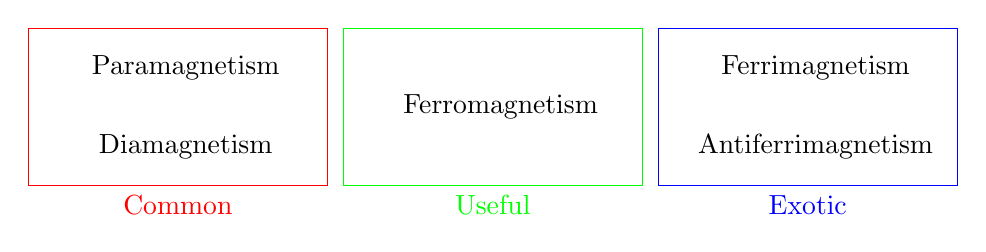
\begin{tikzpicture}
	\node at (0,1) {Paramagnetism};
	\node at (0,0) {Diamagnetism};
	\node at (4,0.5) {Ferromagnetism};
	\node at (8,1) {Ferrimagnetism};
	\node at (8,0) {Antiferrimagnetism};

	\draw[red] (-2,-0.5) rectangle ++ (3.8,2); 
	\draw[green] (2,-0.5) rectangle ++ (3.8,2); 
	\draw[blue] (6,-0.5) rectangle ++ (3.8,2); 

	\draw[red] (-2,-0.5)  -- +(3.8,0) node[midway, below]{Common};
	\draw[green] (2,-0.5)  -- +(3.8,0) node[midway, below]{Useful};
	\draw[blue] (6,-0.5)  -- +(3.8,0) node[midway, below]{Exotic};
\end{tikzpicture}
\end{center}

\subsubsection{The Big Two: Diamagnetism and Paramagnetism}
The big two types of magnetism that most materials exhibit are diamagnetism and paramagnetism.
"dia-" is a prefix meaning through and "para-" is a prefix meaning alongside or near, 
these prefixes are related to how magnetic field lines interact with the material and will be useful later.
\\

When an external magnetic field is applied a diamagnetic material has an induced field opposing the external field and feels a repulsive force from it.
When an external magnetic is applied a paramagnetic material has an induced field aligning with the external field and feels an attractive force to it.
Neither material keeps this induced field once the external field is removed.
\\

Along side being the most simple behavior most materials exhibit one of these forms of magnetism,
although the strength is often so low that it can't be felt in normal life.
The rule of thumb is that if all the electrons of a material are paired than it is diamagnetic,
if there are unpaired electrons it is paramagnetic.
\\

Interestingly, all materials spontaneously exhibit some diamagnetism to some degree with paramagnetism only being felt when it overcome the repulsion.
There are two ways to think about why diamagnetism is so common and the default:
\begin{enumerate}
\item Induced magnetic field naturally oppose the inducing fields.
\item Because the electromagnetic force is so strong thing we interact with are likely near some type of stable equilibria and therefore oppose change.
\end{enumerate}

\subsubsection{The Center of Attention: Ferromagnetism}
Above a specific temperature a ferromagnetic material act paramagnetically,
bellow that temperature the magnetic moments of the material are able to stay ordered and aligned even when an external field is removed.
The specific temperature of a ferromagnetic material around which this behaviour is exhibited is called the Curie temperature.
\\

Ferromagnetic material behave like the colloquial meaning of the word magnetic and most things you'll call a magnet is a ferromagnet.
For example, a lodestone is a ferromagnet.

\subsubsection{The Weird Two: (Anti-)Ferrimagnetism}
Ferrimagnetism and antiferrimagnetism are able to keep their magnetic moments aligned in the absence of an external magnetic field.
The temperature bellow which they do this is called the Curie temperature for ferrimagnetism and Néel temperature for antiferrimagnetism.
Like ferromagnetism, above these temperatures they act paramagnetic. 
\\

The difference is that ferromagnetism has all the persistent magnetic moment aligned in the same direction,
in ferrimagnetism there are different moments aligned in different directions but still an net magnetic moment.
In antiferrimagnetism the moments are persistent but cancel out to no net magnetic moment.
\\

Examples of both include crystals with two moments in the unit cell.
Chromium is an example of an antiferrimagnetic material,
although I can't think of how its or any other material's antiferrimagnetism affect daily life.
\\

Most items that are ferromagnetic are actually ferrimagnetic because there's usually at least one component of the material that oppositely aligned to the net moment.
Hence the examples from the ferromagnetism section actually apply here. 

\subsection{Quantum Foundations}
The fundamental magnetic quantum property is that electrons have an innate magnetic moment $\mu$ related to total angular momentum $L$ by:
\[\mu = -\frac{e}{2m_e}L\]
Where $e$ it the electrons charge and $m_e$ is the electrons mass.
Recall that the total angular momentum has both spin and orbital components.
\\

We now consider a common Hamiltonian form for multi-electron systems:
\[H = H_\text{Strong} + H_\text{Weak} + \sum_{i\neq j}a_{i,j}\mu_i\cdot \mu_j +B\cdot\sum_i\mu_i\]
Where $\mu_i$ is the magnetic moment of the $i^\text{th}$ electron,
$B$ is an external magnetic field,
$H_\text{Strong}$ is a dominating term that doesn't depend on $\mu_i$ (such as electric repulsion),
$H_\text{Weak}$ is a dominated term that may depend on $\mu_i$,
and $a_{i,j}$ is the coupling between the magnetic moments of the $i^\text{th}$ and $j^\text{th}$ electrons.

\subsubsection{Dia and Para Magnetism:}
This Hamiltonian explains a lot of the dia and para magnetic properties discussed earlier,
discarding the weak $H_\text{Weak}$ term we see that magnetic properties mainly come from the last terms:
\[\sum_{i\neq j}a_{i,j}\mu_i\cdot \mu_j +B\cdot\sum_i\mu_i\]
Which,
in the absence of an external magnetic field,
we would expect the magnetic moments to arrange themselves such that the first term is minimized.
\\

Minimizing the first term is easy if the electrons can be paired,
meaning there are an even number of electrons and each electron is coupled with only one other electron and that electron is in turn coupled only with the first,
since we can simply make sure each set of paired electrons have opposite magnetic movements so the contribution of this term is zero.
When an external field is applied it has to overcome this ideal arrangement and once the external field is removed it would be expected to return to this arrangement.
Hence materials with paired electrons are diamagnetic.
\\

Even without this perfect pairing the external magnetic field has to overcome some minimizing arrangements,
which is why all materials are diamagnetic to some degree,
but when common materials doesn't have paired electrons they most commonly has some paired electrons and one or more completely uncoupled electrons.
These uncoupled electrons don't contribute to the first term they are free to align with an external magnetic field in the second,
reducing the combined terms and causing paramagnetic behaviour.
\\

Note that when the external field is removed the uncoupled electrons will likely misalign naturally.
Either because of instead being completely uncoupled there is slight coupling with themselves and other electrons and hence have a tendency to misalign to minimize the first term.
Or that as an statistical ensemble the net polarization will be zero through entropy,
as there's nothing favouring alignment.

\subsubsection{Other Magnetic Behaviour}
\begin{center}
\begin{tikzpicture}
	% Levels
	\draw  (1,2) node[left] {$E_0$}--(3,2);
	\draw  (4,3)-- +(2,0) node [midway] {$\big\uparrow\big\uparrow$};
	\draw  (4,1)-- +(2,0) node [midway] {$\big\uparrow\big\downarrow$};
	\draw  (7,3)-- +(2,0) node [midway] {$\big\downarrow\big\downarrow$};
	\draw  (7,1)-- +(2,0) node [midway] {$\big\downarrow\big\uparrow$};

	% Links
	\draw [blue, dashed] (3,2) -- (4,3);
	\draw [blue, dashed] (3,2) -- (4,1);
	\draw [blue, dashed] (6,3) -- (7,3);
	\draw [blue, dashed] (6,1) -- (7,1);
\end{tikzpicture}

Naïve Energy Level Diagram for a Two Electron System.
\end{center}
While this Hamiltonian easily explains dia and para magnetism,
both of which lose their field when the external field is is removed,
if interpreted naïvely it can have trouble explaining how any material can maintain an internal field when the external field is removed.
The interpretations goes like this:
{\em "Consider the energy levels determined by $H_\text{Strong}$.
When the external field is removed these energy levels would split based largely on the coupling term.
When the magnetic moments are misaligned the coupling term would be minimized and hence be the ground state.
Hence the material would not keep an internal field."}

\subsection{Exchange Interaction}
What this naïve interoperation ignores is spin statistics and their effects on indistinguishable particles.
A sketch of the principle is this, 
let a wave function, $\psi(r,s)$, be dependent of the two identical particles $r$ and $s$.
Since they are indistinguishable we must get the same probability function when the arguments are swapped:
\[|\psi(r,s)|^2=|\psi(s,r)|^2\]
For this to be true for all $r$ and $s$ we require:
\[\psi(r,s) = k\psi(s,r)\quad\text{where}\quad |k|^2=1\]
Whose solutions are:
\[k=+1\quad\text{(Symmetric)}\quad k=-1\quad\text{(Antisymmetric)}\]
Electrons are fermions which are known to be antisymmetric meaning the wave function of two electrons must be antisymmetric. 
With this knowledge lets return to the naïve interpretations.
$H_\text{Strong}$ does produce energy levels independent of $\mu_i$ but that doesn't mean when it comes splitting we can choose $\mu_i$ as we please.
Instead $\mu_i$ must be chosen such that the wave functions for that energy level are antisymmetric.
This is called the exchange interaction\footnote{Formerly and commonly called the exchange force but this name is discouraged as it is in no technical way analogous to a force.} and provides a mechanism through which an internal field persist in the ground state.

\subsubsection{Example: Hydrogen Gas}
\begin{center}
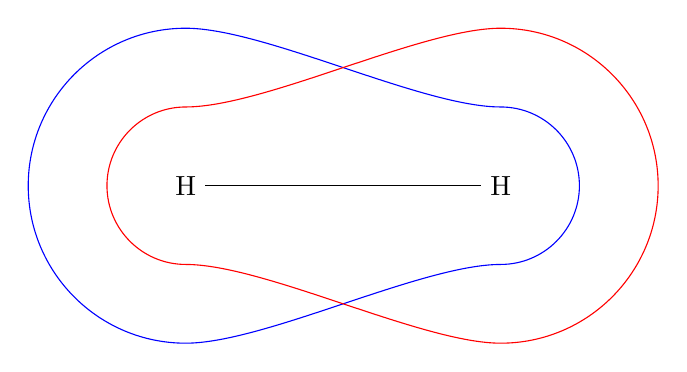
\begin{tikzpicture}
	\draw (-2,0) node[fill=white]{H} -- (2,0) node[fill=white]{H};
	\draw (-2,2)[blue] arc(90:270:2)
	.. controls +(1,0) and +(-1,0) .. (2,-1)
	arc(-90:90:1)
	.. controls +(-1,0) and +(1,0) .. (-2,2);

	\draw (-2,1)[red] arc(90:270:1)
	.. controls +(1,0) and +(-1,0) .. (2,-2)
	arc(-90:90:2)
	.. controls +(-1,0) and +(1,0) .. (-2,1);
\end{tikzpicture}

Representation of Hydrogen Gas with \\Two Single Electron Ground States Shown.
\end{center}
A common example of the exchange interaction is the ground state of hydrogen gas\footnote{Sometimes called "hydrogenic atoms" since,
despite commonly being a gas,
we don't have to assume so for the quantum analysis.}.
For reasons outside the scope of this example,
the ground states for hydrogen gas with a single electron are known to be spanned by two wave functions,
both independent of spin,
where the electron favours one atom more than another but are otherwise similar.
To analyse the ground state for hydrogen gas with two electrons it makes sense to consider combinations of these wave functions:
\[\ket{1,1},\,\ket{1,2},\,\ket{2,1},\,\ket{2,2}\]
Where $\ket{1,2}$ is the wave function where the first electron is closer to the first atom and the second electron is closer the second atom and likewise for other states.
The combination of these states with minimal energy is given by:
\[\frac{1}{\sqrt{2}}(\ket{2,1}+\ket{1,2})\]
A symmetric function.
If we similarly let $\ket{\uparrow,\downarrow}$ be the spin state were the first electron is up and the second is down we can write all our spin options for two electrons as:
\[\left.\begin{matrix}\ket{\uparrow,\uparrow}\\\frac{1}{\sqrt{2}}(\ket{\uparrow,\downarrow}+\ket{\downarrow,\uparrow})\\\ket{\downarrow,\downarrow}\end{matrix}\right\}\text{Symmetric}\quad\quad\frac{1}{\sqrt{2}}(\ket{\uparrow,\downarrow}-\ket{\downarrow,\uparrow})\bigg\}\text{Antisymmetric}\]
Noticing that there's only one antisymmetric spin option to get an antisymmetric total wave function from our symmetric spinless wave function our only choice is:
\[\frac{1}{2}(\ket{\uparrow,\downarrow}-\ket{\downarrow,\uparrow})(\ket{2,1}+\ket{1,2})\]
Hence despite the ground state seemingly not putting any requirements on spin a requirements arises from the spin statistics of indistinguishable particles which does.
\\

Two quick interesting notes to include here are:
\begin{enumerate}
\item Anyone that enjoyed high-school chemistry should be please to see that we have recovered the idea of a covalent bond between the two hydrogen.
As the ground state of two first group elements being two electrons of in opposite spin being shared between them.
\item I'm being somewhat lose when saying "spinless wave function". 
What I technically mean is that if our total wave function belongs to the vector space $V$ and our available spins form the space $S$ then our spinless wave function is from a space $W$ such that $V=S\otimes W$.
This works because our space of wave functions happen to be independent of spin meaning we can factorize $V$ into such a form.
This also means that the multiplication in our final expression is actually the tensor product.
\end{enumerate}

%% A Draft for the Exchange Interaction that I ended up not liking enough to continue with, but also didn't want to delete.
% 
% \subsection{Exchange Interaction Draft}
% Let $\ket{\Phi_1}$ and $\ket{\Phi_2}$ be wave functions for indistinguishable particles that include spin.
% We express these states in the position-spin base in the standard way:
% \[\ket{\Phi_n} = \int\Phi_n(r_n)\ket{s_n,r_n}\,dr_n\]
% Observe that theres no summation over $s_n$ since it is fixed for each $\ket{\Phi_n}$.
% It could be included anyway and just zero half the coefficients,
% but I find that too messy.
% \\
% 
% Construct basis for the combined systems through the standard:
% \[\ket{s_1,s_2,r_1,r_2} = \ket{s_1,r_1}\otimes\ket{s_2,r_2}\]
% We can get some immediate results from just by analysing the basis, let:
% \begin{equation*}
% \begin{aligned}
% \hat{P}_s\ket{s_1,s_2,r_1,r_2} =& k_s\hat{P}_s\ket{s_2,s_1,r_1,r_2}\\ 
% \hat{P}_r\ket{s_1,s_2,r_1,r_2} =& k_r\hat{P}_s\ket{s_1,s_2,r_2,r_1}\\ 
% \hat{P}\ket{s_1,s_2,r_1,r_2} =& k\hat{P}_s\ket{s_1,s_1,r_2,r_1}\\ 
% \end{aligned}
% \end{equation*}
% The last operator is swapping the two indistinguishable particles and hence is governed by standard exchange symmetry, meaning $k=1$ for bosons and $k=-1$ for fermions. 
% 
% The other operators swap just position and spin and are governed by similar rules.
% To see why observe that the left and right states have the same observables,
% hence the operators are unitary,
% but the operators are also involuntary:
% \[\hat{P}_s^2 = \hat{P}_r^2 = I\]
% This means:
% \[\ket{s_1,s_2,r_1,r_2} = \hat{P}_s^2\ket{s_1,s_2,r_1,r_2}=k_s^2\ket{s_1,s_2,r_1,r_2}\]
% Requiring $k_s = \pm 1$,
% and likewise for $k_r$.
% 
% Let $\hat{H}_1$ and $\hat{H}_2$ be operators for the respective states.
% Define a new operator:
% \[\hat{H} = \hat{H}_1\otimes I + I\otimes\hat{H}_2+\hat{H}_{12}\]
% Where $\hat{H}_{12}$ is the "interaction" term.
% 
% \subsection{Future Plans}
% Clebsch–Gordan coefficients and triplet states
% \[\bra{\Phi_\pm}H\ket{\Phi_\pm} = \frac{1}{2}\bigg(\bra{\Phi_+}H\ket{\Phi_+}+\bra{\Phi_-}H\ket{\Phi_-}\bigg)\pm\frac{1}{2}\bigg(\bra{\Phi_+}H\ket{\Phi_+}-\bra{\Phi_-}H\ket{\Phi_-}\bigg)\]
% Non-separable, no classic interpretation.
% Magnetite and lodestone
% Open problem, clearly not from another magnetic but from an current induced field.
% Not made from another magnet Earths magnetic field is likely too weak, maybe lightning bolt
%\begin{center}
%\begin{tikzpicture}
%	% E_0 Levels
%	\draw [red] (1,2) node[left] {$E_0$}--(3,2);
%	\draw [red] (4,3)--(6,3) node [midway] {$\big\uparrow\big\uparrow$};
%	\draw [red] (4,1)--(6,1) node [midway] {$\big\uparrow\big\downarrow$};
%	\draw [red] (7,3)--(9,3) node [midway] {$\big\downarrow\big\downarrow$};
%	\draw [red] (7,1)--(9,1) node [midway] {$\big\downarrow\big\uparrow$};
%
%	% E_0 links
%	\draw [blue, dashed] (3,2) -- (4,3);
%	\draw [blue, dashed] (3,2) -- (4,1);
%	\draw [blue, dashed] (6,3) -- (7,3);
%	\draw [blue, dashed] (6,1) -- (7,1);
%
%	% E_1 Levels
%	\draw [red] (1,7) node[left] {$E_1$}--(3,7);
%	\draw [red] (4,8)--(6,8) node [midway] {$\big\uparrow\big\uparrow$};
%	\draw [red] (4,6)--(6,6) node [midway] {$\big\uparrow\big\downarrow$};
%	\draw [red] (7,8)--(9,8) node [midway] {$\big\downarrow\big\downarrow$};
%	\draw [red] (7,6)--(9,6) node [midway] {$\big\downarrow\big\uparrow$};
%
%	% E_1 links
%	\draw [blue, dashed] (3,7) -- (4,8);
%	\draw [blue, dashed] (3,7) -- (4,6);
%	\draw [blue, dashed] (6,8) -- (7,8);
%	\draw [blue, dashed] (6,6) -- (7,6);
%\end{tikzpicture}
%
%Naïve Energy Level Diagram
%\end{center}
%\[\left.\begin{matrix}\ket{1,1}\\\frac{1}{\sqrt{2}}(\ket{1,2}+\ket{2,1})\\\ket{2,2}\end{matrix}\right\}\text{Symmetric}\quad\quad\frac{1}{\sqrt{2}}(\ket{1,2}-\ket{2,1})\bigg\}\text{Antisymmetric}\]
